\documentclass[12pt]{article}
\usepackage{sbc-template}
\usepackage{graphicx,url}
\usepackage[utf8]{inputenc}
\usepackage[brazil]{babel}
\usepackage{float}
\usepackage{booktabs}

\title{Rastreamento de Objetos Baseado em Casamento de Padrões (Template Matching): Uma Abordagem Simplória utilizando OpenCV}

\author{Herton Silveira\inst{1}, Diogo Silva de Carvalho\inst{1}, Andre Vinicius Trentini\inst{1}}

\address{Professor Orientador: Gilmário Barbosa dos Santos}

\begin{document}

\maketitle

\begin{abstract}
This article describes the implementation and analysis of a simple object tracking strategy in video using Template Matching techniques available in the OpenCV library. From a short video containing 300 frames, with a static camera and no autofocus, the first frame was extracted and a region of interest (ROI) was cropped as a template. Six matching methods (TM\_SQDIFF, TM\_SQDIFF\_NORMED, TM\_CCORR, TM\_CCORR\_NORMED, TM\_CCOEFF, and TM\_CCOEFF\_NORMED) were tested to identify the target in each frame. The analysis revealed that the TM\_CCOEFF\_NORMED method has the best discrimination capacity and stability for the scene in question.
\end{abstract}

\begin{resumo}
Este artigo descreve a implementação e análise de uma estratégia simples de rastreamento de objetos em vídeo utilizando técnicas de Template Matching (casamento de padrões) disponíveis na biblioteca OpenCV. A partir de um vídeo curto contendo 300 quadros, com câmera estática e sem autofoco, foi extraído o primeiro quadro e recortada uma região de interesse (ROI) como template. Seis métodos de matching (TM\_SQDIFF, TM\_SQDIFF\_NORMED, TM\_CCORR, TM\_CCORR\_NORMED, TM\_CCOEFF e TM\_CCOEFF\_NORMED) foram testados para identificar o alvo em cada quadro. Os resultados foram tabelados e plotados graficamente, sendo as métricas comparadas por meio de estatística descritiva (média, desvio padrão e coeficiente de variação). A análise revelou que o método TM\_CCOEFF\_NORMED possui a melhor capacidade de discriminação e estabilidade para a cena em questão e, por isso, foi o método escolhido para gerar o vídeo de saída com o rastreio marcado.
\end{resumo}

\section{Introdução}
O rastreamento de objetos em sequências de imagens (\textit{surveillance} / monitoramento) é uma tarefa fundamental em visão computacional. Consiste em determinar a trajetória e garantir a identificação de um ou mais objetos ao longo do tempo. Existem diversas abordagens consolidadas para obter um rastreio, tais como o uso do fluxo ótico na estimativa de movimento ou detectores robustos de características (SURF, ORB, BRIEF).

No entanto, uma forma inicial e bastante didática de se realizar um rastreio é aplicar uma técnica de detecção de Regiões de Interesse (ROI - \textit{Regions of Interest}) através da avaliação de casamento (\textit{matching}) de um padrão (\textit{template}) isolado na primeira cena em relação a cada um dos quadros subsequentes de um vídeo. O objetivo deste trabalho é exercitar o método de \textit{Template Matching} por meio da biblioteca OpenCV (\texttt{cvMatchTemplate}), comparar e interpretar as diferentes abordagens matemáticas disponíveis na biblioteca e eleger a melhor para construir um algoritmo de rastreamento funcional.

\section{Fundamentação Teórica}
A essência do \textit{Template Matching} baseia-se em deslizar um recorte de padrão (\textit{template}) de dimensões $w \times h$ sobre uma imagem original e realizar o cômputo matemático em cada posicionamento possível para definir o ``casamento''. O OpenCV gerencia essa tarefa através da função \texttt{cv2.matchTemplate()}. O resultado dessa função é um mapa em tons de cinza descrevendo o quão semelhante uma sub-região da imagem é ao \textit{template}. 

Existem diversas estratégias para calcular essa relação:
\begin{itemize}
    \item \textbf{Diferença Quadrada (TM\_SQDIFF e TM\_SQDIFF\_NORMED)}: A função calcula a diferença ao quadrado entre os pixels do template e os da imagem. Sendo uma medida de distância, o melhor casamento é o valor mais baixo possível (tendendo a zero).
    \item \textbf{Correlação Cruzada (TM\_CCORR e TM\_CCORR\_NORMED)}: A função multiplica de maneira cruzada as intensidades dos pixels. Valores altos indicam excelentes casamentos.
    \item \textbf{Coeficiente de Correlação (TM\_CCOEFF e TM\_CCOEFF\_NORMED)}: O método também realiza multiplicação cruzada, mas realiza a subtração da média previamente (\textit{mean-removed}). Consequentemente, um casamento perfeito atinge o valor máximo disponível, um mau casamento tem valor nulo, e uma correspondência perfeitamente invertida apresenta um valor negativo.
\end{itemize}

As versões normalizadas (\texttt{NORMED}) dessas equações reajustam os dados resultantes para o intervalo genérico de $[0, 1]$ ou $[-1, 1]$. Essa técnica facilita a interpretação em qualquer ambiente de iluminação e permite a configuração de limiares automáticos e generalistas.

\section{Metodologia}
Para o projeto simulado de rastreamento, os seguintes processos foram conduzidos através de código na linguagem Python em associação aos métodos do OpenCV:
\begin{enumerate}
    \item \textbf{Captura do Vídeo}: Foi desenvolvido e utilizado um vídeo caseiro contemplando aproximadamente 300 quadros. O deslocamento do objeto ocorreu vagarosamente frente a um fundo estático e inalterado.
    \item \textbf{Separação de Quadros}: Os quadros individuais do vídeo foram segmentados e convertidos para o formato de tons de cinza, resultando nas imagens individuais em disco.
    
    Exemplos de quadros capturados ao longo do tempo da gravação original podem ser observados na Figura~\ref{fig:frames}.
    
    \begin{figure}[H]
        \centering
        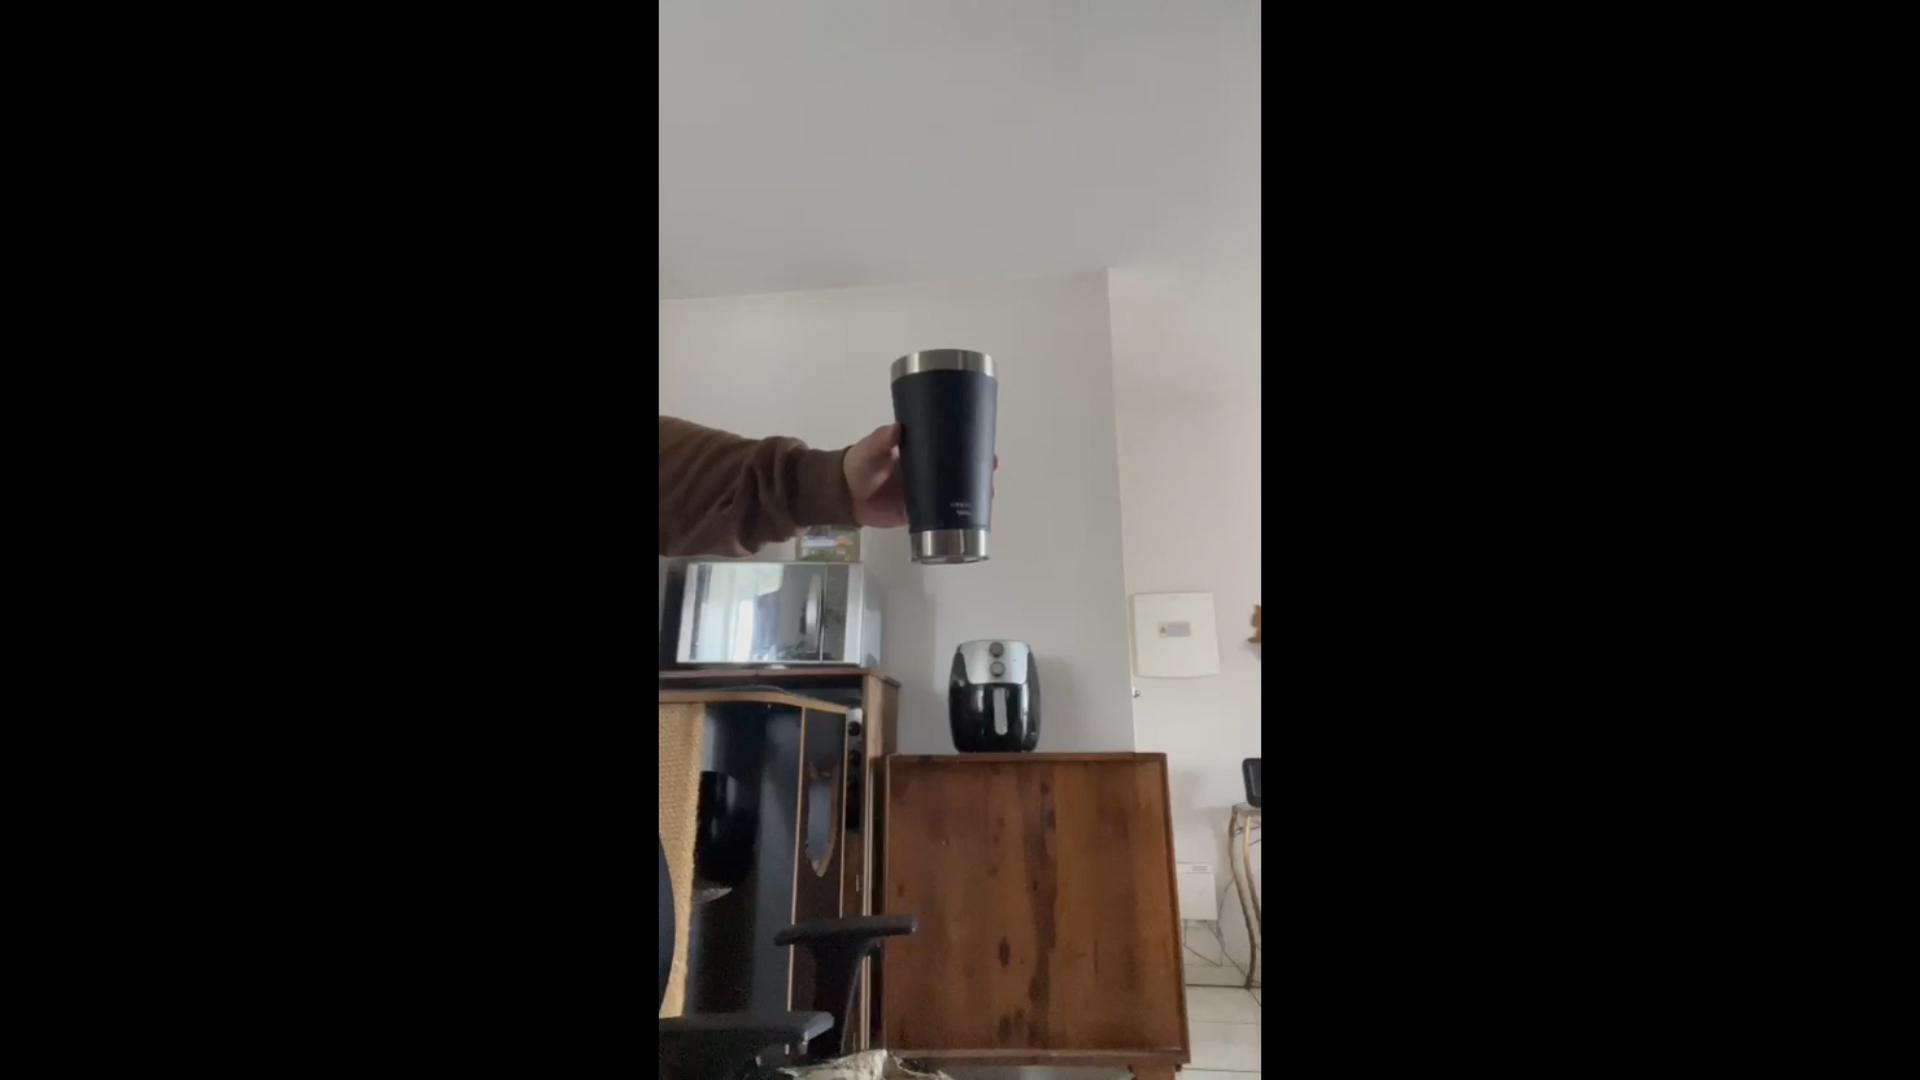
\includegraphics[width=0.32\textwidth]{videoPIM_2_frame_00000.png}
        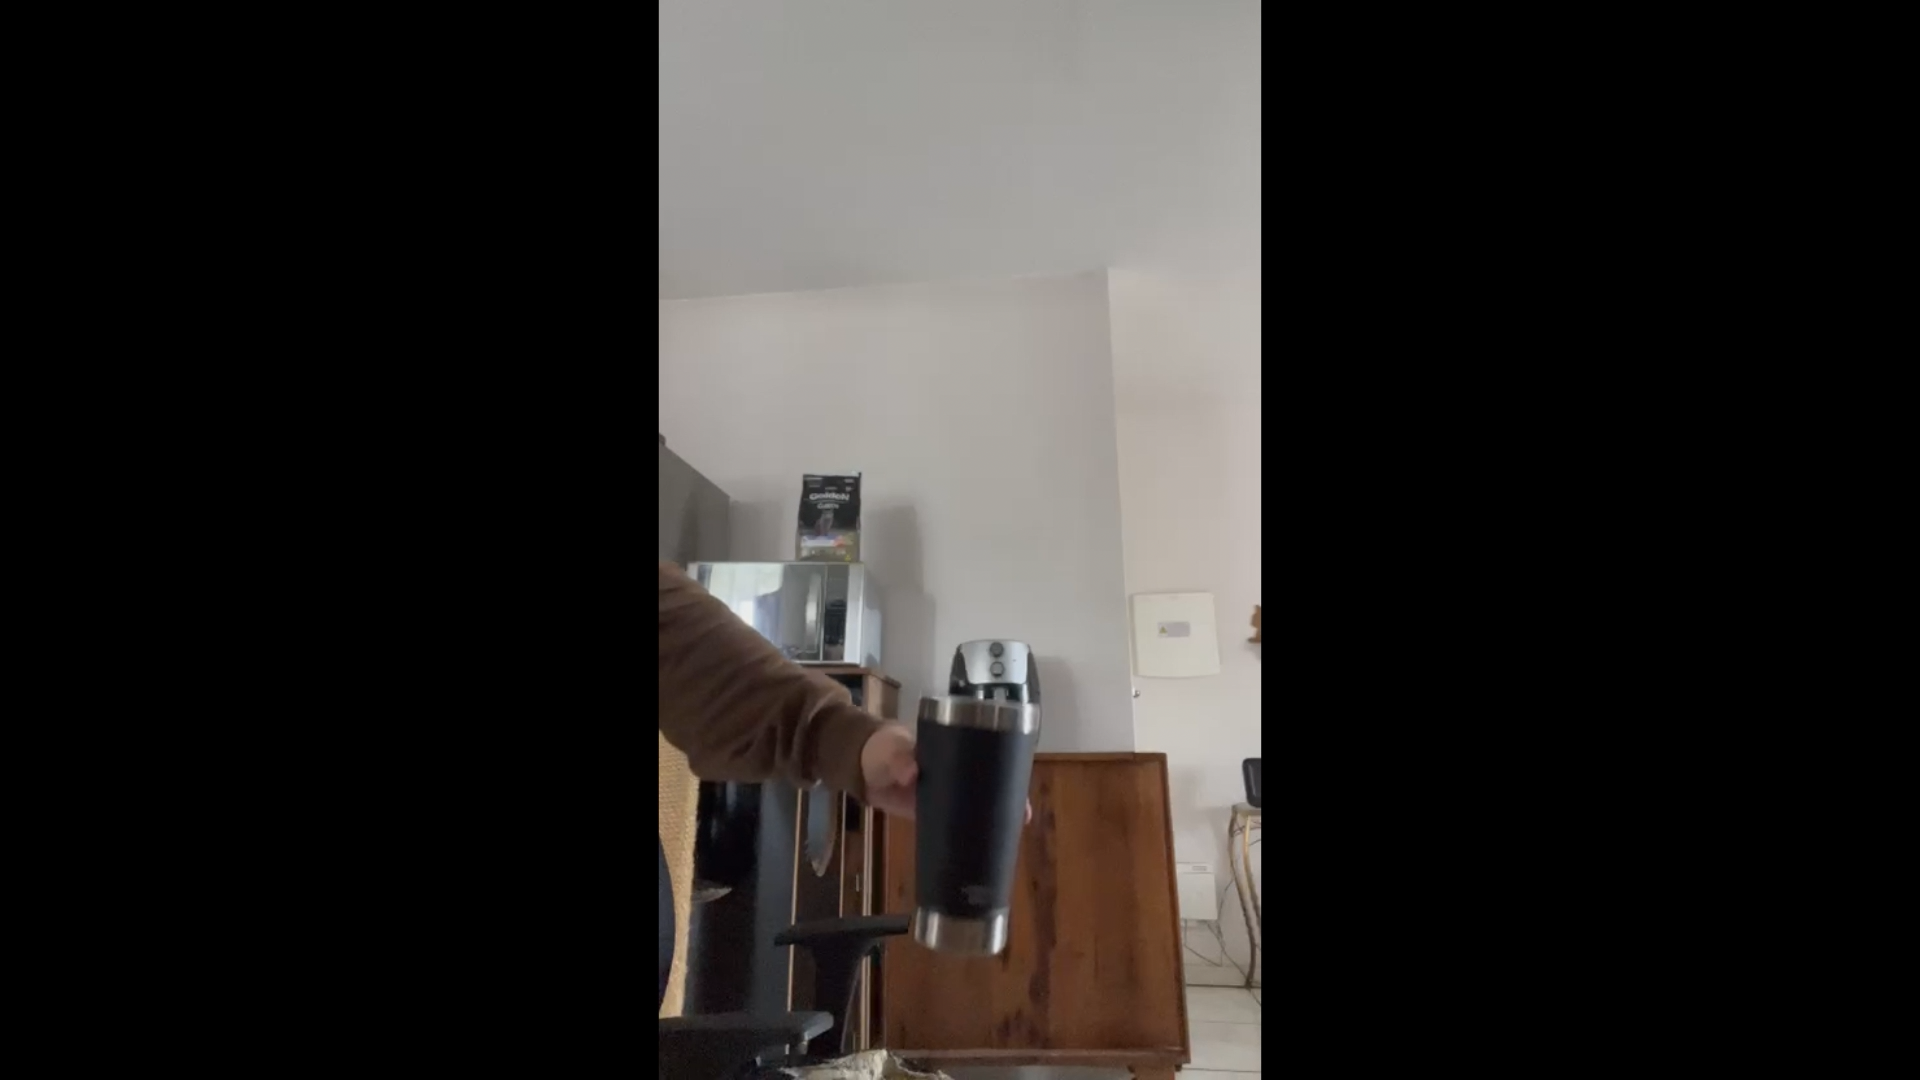
\includegraphics[width=0.32\textwidth]{videoPIM_2_frame_00150.png}
        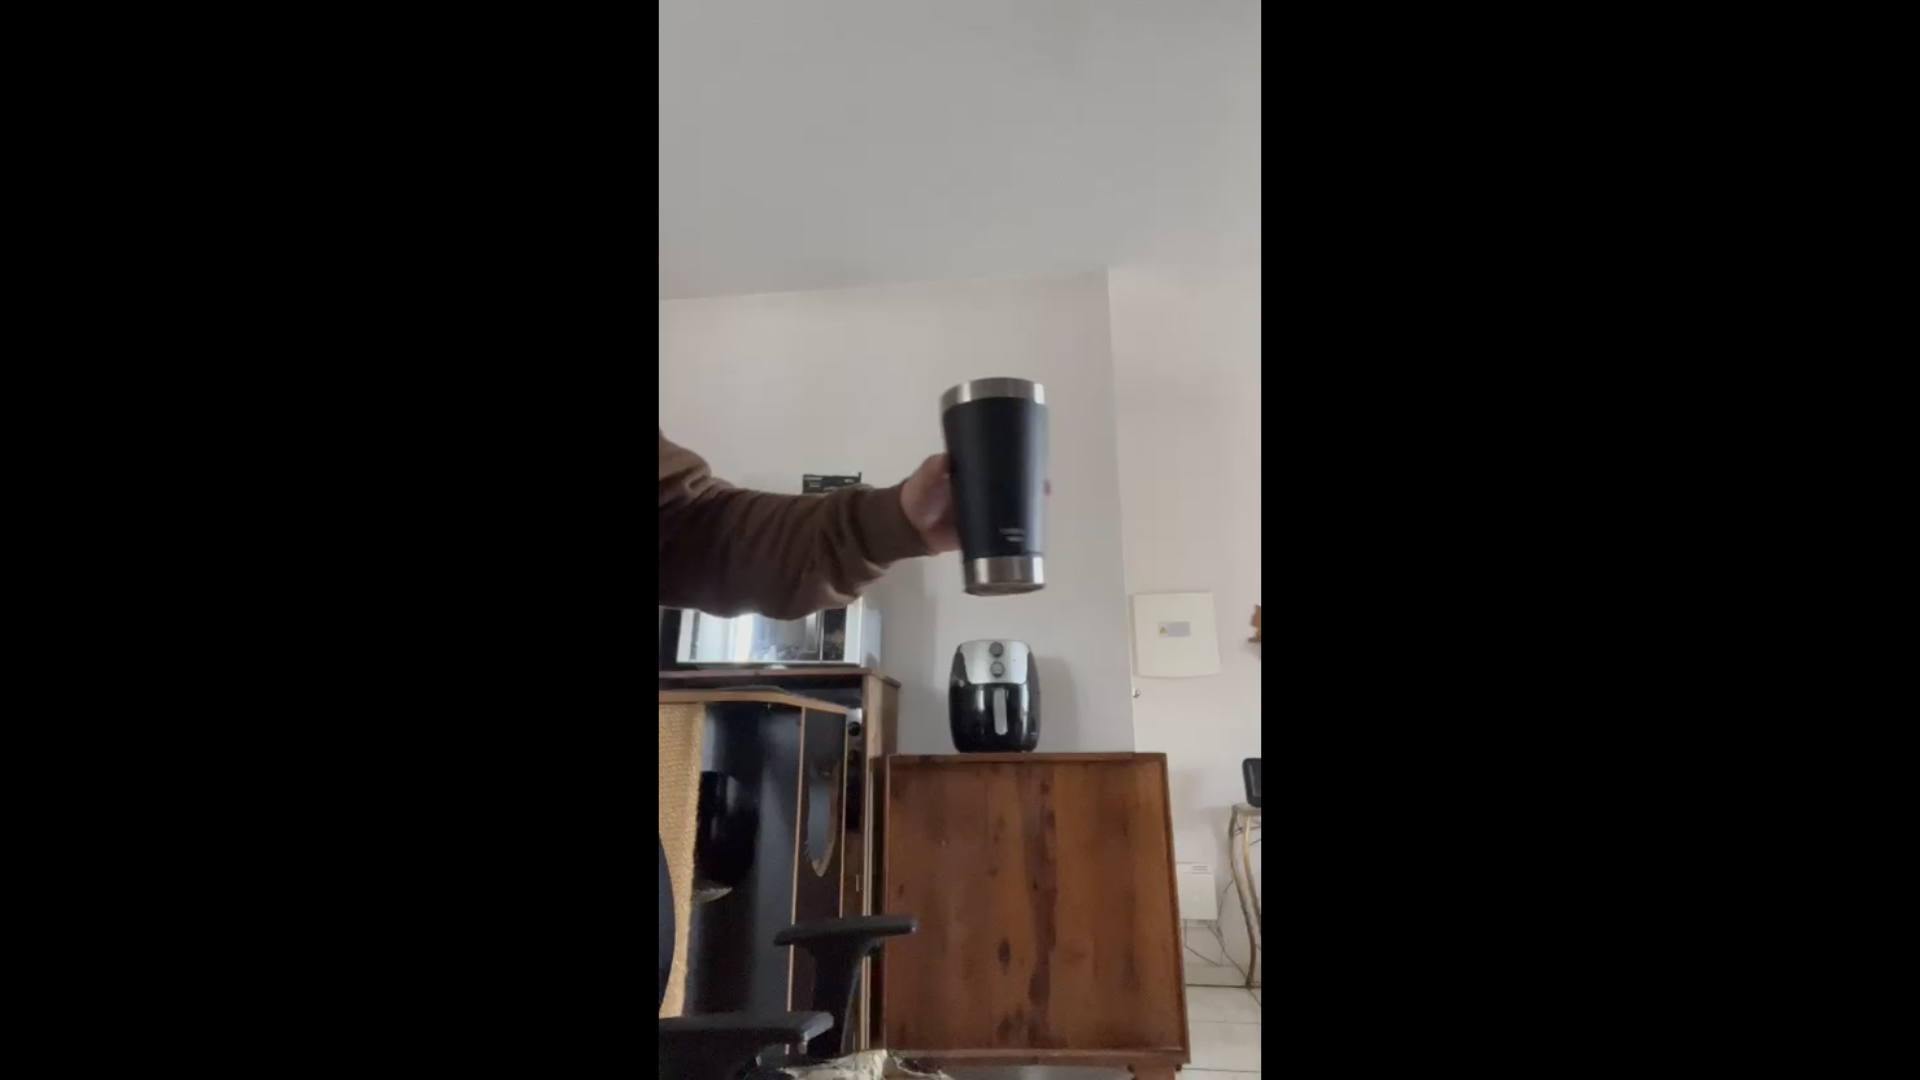
\includegraphics[width=0.32\textwidth]{videoPIM_2_frame_00299.png}
        \caption{Quadro Inicial, Quadro Intermediário e Quadro Final.}
        \label{fig:frames}
    \end{figure}

    \item \textbf{Obtenção do Template}: Mediante interatividade providenciada pela função \texttt{cv2.selectROI()}, selecionou-se manualmente uma amostra na primeira imagem contemplando o enquadramento ideal do objeto a ser rastreado, definindo assim o template base.
    \item \textbf{Aplicação dos Métodos de Matching}: Aplicou-se um iterador em todos os quadros e testou-se cada um dos seis métodos. Capturaram-se os menores e maiores valores resultantes através do método \texttt{cv2.minMaxLoc()}. 
    \item \textbf{Geração de Análise}: As referências coletadas foram ordenadas e salvas em planilhas CSV e traçadas em gráficos para elucidação de desempenho.
    \item \textbf{Vídeo Resultante}: Uma vez selecionado o algoritmo de maior confiabilidade, gerou-se um arquivo final no formato MP4 desenhando-se as caixas de identificação para demarcar a silhueta encontrada ao longo do trajeto no vídeo.
\end{enumerate}

\section{Resultados e Discussão}
Para avaliar a assertividade de cada estratégia, traçou-se e exportou-se os valores limítrofes encontrados durante todos os 300 quadros de simulação para cada método. As figuras a seguir representam visualmente as avaliações de respostas extremas das funções.

\begin{figure}[H]
    \centering
    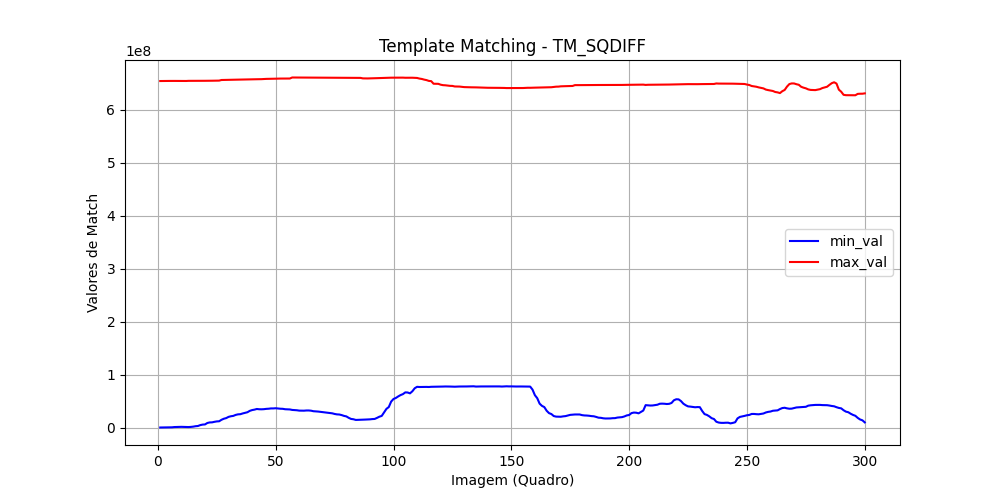
\includegraphics[width=0.48\textwidth]{grafico_TM_SQDIFF.png}
    
\includegraphics[width=0.48\textwidth]{grafico_TM_SQDIFF_NORMED.png}
    \caption{Diferença Quadrada (Esquerda) e Diferença Quadrada Normalizada (Direita).}
\end{figure}

\begin{figure}[H]
    \centering
    
\includegraphics[width=0.48\textwidth]{grafico_TM_CCORR.png}
    
\includegraphics[width=0.48\textwidth]{grafico_TM_CCORR_NORMED.png}
    \caption{Correlação Cruzada (Esquerda) e Correlação Cruzada Normalizada (Direita).}
\end{figure}

\begin{figure}[H]
    \centering
    
\includegraphics[width=0.48\textwidth]{grafico_TM_CCOEFF.png}
    
\includegraphics[width=0.48\textwidth]{grafico_TM_CCOEFF_NORMED.png}
    \caption{Coeficiente de Correlação (Esquerda) e Coeficiente Normalizado (Direita).}
\end{figure}

Foi processada a análise estatística sobre o volume de dados resgatados das planilhas CSV, obtendo-se o quadro comparativo descrito na Tabela~\ref{tab:estatisticas}.

\begin{table}[H]
    \centering
    \caption{Resultados Estatísticos dos Métodos Avaliados}
    \vspace{0.2cm}
    \resizebox{\textwidth}{!}{
    \begin{tabular}{llcccc}
        \toprule
        \textbf{Método} & \textbf{Métrica usada} & \textbf{Média} & \textbf{Desvio padrão} & \textbf{CV (\%)} & \textbf{Faixa de valores} \\
        \midrule
        TM\_CCOEFF & max\_val & $5,26\times10^{7}$ & $3,15\times10^{6}$ & 6,0 & não normalizado \\
        TM\_CCOEFF\_NORMED & max\_val & 0,861 & 0,064 & 7,5 & [-1, 1] \\
        TM\_CCORR & max\_val & $2,97\times10^{8}$ & $5,72\times10^{6}$ & 1,9 & não normalizado \\
        TM\_CCORR\_NORMED & max\_val & 0,949 & 0,026 & 2,7 & [0, 1] \\
        TM\_SQDIFF & min\_val & $1.89\times10^{7}$ & $1.14\times10^{7}$ & 60,0 & não normalizado \\
        TM\_SQDIFF\_NORMED & min\_val & 0,118 & 0,068 & 58,2 & [0, 1] \\
        \bottomrule
    \end{tabular}}
    \label{tab:estatisticas}
\end{table}

\subsection{Análise e Justificativa de Melhor Método}
\textbf{Métodos de Diferença Quadrada (TM\_SQDIFF e TM\_SQDIFF\_NORMED):} Estes métodos apresentaram o maior coeficiente de variação ($\approx 60\%$), perceptível também pelos ruídos irregulares plotados na linha de valor mínimo em seus respectivos gráficos. Isto sinaliza uma altíssima sensibilidade a qualquer mudança singela do cenário. Por carecer de ajustes de normalização no contraste da matriz analítica, são altamente afetados pelas variações de brilho entre os quadros.

\textbf{Métodos de Correlação (TM\_CCORR E TM\_CCORR\_NORMED):} Exibiram a menor variação entre todos do experimento ($\approx 2\% - 3\%$). Porém, este comportamento aparentemente estável reflete sua ineficiência central: métodos puros de correlação cruzada não realizam subtração das médias do entorno. Desse modo, o valor obtido é corrompido por regiões de brilho exagerado, inviabilizando a avaliação real dos contornos do objeto.

\textbf{Métodos de Coeficiente de Correlação (TM\_CCOEFF e TM\_CCOEFF\_NORMED):} Este grupo ofereceu maior equilíbrio para o projeto. Por subtraírem a média de luminância das superfícies antes de correlacioná-las pontualmente, resultam em robustez contra cenários instáveis e reflexos inconstantes. O TM\_CCOEFF\_NORMED espelha o Coeficiente de Correlação de Pearson, facilitando sobremaneira estipular barreiras seguras na análise do sistema.

Sendo assim, o \texttt{TM\_CCOEFF\_NORMED} foi atestado como a vertente de maior confiabilidade na tarefa e foi o algoritmo selecionado para processar a re-construção das marcações de limite no objeto alvo renderizadas no arquivo audiovisual conclusivo.

\section{Conclusão}
O procedimento delineado nesta pesquisa permitiu realizar e comparar sistematicamente abordagens basilares de rastreamento contínuo em vídeo a partir da manipulação do OpenCV no ecossistema de Python. O experimento apontou na prática que algoritmos de Template Matching não subtraídos de sua média local sucumbem facilmente aos níveis flutuantes de energia luminosa. Por outro lado, a detecção refinada por métricas correlacionais normalizadas (TM\_CCOEFF\_NORMED) revelou um processamento preciso, seguro e de fácil delimitação parametrizada, evidenciando sua capacidade educacional e funcionalidade objetiva no campo da Visão Computacional.

\begin{thebibliography}{9}

\bibitem{opencv_template_matching}
OPENCV.
\textit{Template Matching}. Documentation.
Disponível em: \url{https://docs.opencv.org/4.5.2/d4/dc6/tutorial_py_template_matching.html}.
Acesso em: 20 Set. 2026.

\bibitem{opencv_template_matching_34}
OPENCV.
\textit{Template Matching (3.4)}. Documentation.
Disponível em: \url{https://docs.opencv.org/3.4/de/da9/tutorial_template_matching.html}.
Acesso em: 20 Set. 2026.

\bibitem{santos_rastreio}
SANTOS, Gilmário Barbosa dos.
\textit{Rastreio usando matching template}.
Material didático disponibilizado em formato PDF - Aula de PIM.

\end{thebibliography}

\end{document}
